\documentclass[a4paper,12pt]{report}
\usepackage[T2A]{fontenc}
\usepackage[utf8]{inputenc}
%\usepackage[14pt]{extsizes}
\usepackage[english,russian]{babel}
\usepackage {titlesec, textcase} 
\usepackage{amssymb,amsfonts,amsmath,cite,enumerate,float}
\usepackage[dvips]{graphicx}
\usepackage {indentfirst}



% поддержка гиперссылок; гиперссылки в pdf, должен быть последним загруженным пакетом
\ifx\pdfoutput\undefined
    \usepackage[unicode,dvips]{hyperref}
\else
    \usepackage[pdftex,colorlinks,unicode,bookmarks]{hyperref}
\fi

\graphicspath{{images/}}

\makeatletter
\renewcommand{\@biblabel}[1]{#1.} % Заменяем библиографию с квадратных скобок на точку:
\makeatother

% Меняем поля страницы
\usepackage{geometry}
\geometry{left=3cm}
\geometry{right=1.5cm}
\geometry{top=2cm}
\geometry{bottom=2cm}

% Меняем везде перечисления на цифра.цифра
\renewcommand{\theenumi}{\arabic{enumi}}
\renewcommand{\labelenumi}{\arabic{enumi}}
\renewcommand{\theenumii}{.\arabic{enumii}}
\renewcommand{\labelenumii}{\arabic{enumi}.\arabic{enumii}.}
\renewcommand{\theenumiii}{.\arabic{enumiii}}
\renewcommand{\labelenumiii}{\arabic{enumi}.\arabic{enumii}.\arabic{enumiii}.}
\renewcommand{\contentsname}{Содержание}
\renewcommand{\bibname}{Список использованных источников}

\makeatletter
\titleformat{\chapter}{\huge\bfseries}{\thechapter. }{0pt}{\huge}
\makeatother

\begin{document}

\begin{titlepage}
\newpage
\begin{center}
Министерство образования и науки Российской Федерации\\
\vspace{1em} 
Федеральное государственное автономное образовательное учреждение\\
высшего профессионального образования\\
<<Московский физико-технический институт\\
(государственный университет)>>\\
\vspace{1em}
Факультет проблем физики и энергетики\\
\vspace{1em}
Кафедра нелинейных и динамических процессов в астрофизике и геофизике\\
\vspace{5em}
\textbf{\large\MakeTextUppercase{Подготовка программы наблюдений космической миссии "Спектр-УФ": отбор кандидатов в звёзды типа Т Тельца в созвездии Змеи}}\\
\vspace{1em}
Выпускная квалификационная работа\\
(бакалаврская работа)\\
\vspace{1em}
Направление подготовки 03.03.01 Прикладные математика и физика\\
\end{center}
\begin{flushleft}
\vspace{3em}
Выполнила:\\
студентка 183 группы \hrulefill Молярова Тамара Сергеевна\\
\vspace{3em}
Научный руководитель:\\
д.ф.-м.н., ведущий научный сотрудник \hrulefill Сачков Михаил Евгеньевич\\
\vspace{\fill}
\end{flushleft}
\begin{center}
Москва 2015
\end{center}
\end{titlepage}

\tableofcontents

\chapter{Введение}


\section{T Tauri звёзды}
Целью данной работы является поиск звёзд, относящихся к определённому классу: звёзд типа Т Тельца. 
Это предшественники звёзд, подобных Солнцу, а также планетарных систем. Поэтому их изучение очень важно для понимания процесса формирования Солнечной системы, её эволюции и образования планет. 

Как молодые звёзды, звёзды типа Т Тельца обнаруживаются в областях звездообразования. Т Тельца, по имени которой назван этот класс звёзд, расположена в 

\section{Изучаемая область}

В данной работе изучается тёмная туманность, находящаяся в созвездии Змея и Орёл (Serpens-Aquila Rift). Межзвёздная среда в ней находится в холодной фазе, то есть состоит из плотных и холодных облаков газа, в основном молекулярного водорода H$_{2}$. Именно из такого вещества формируются звёзды. Существуют исследования, подтверждающие, что в этой туманности происходит активное звездообразование [Far-ultraviolet Observation of the Aquila Rift with FIMS SPEAR].

\begin{figure}[h]
\center{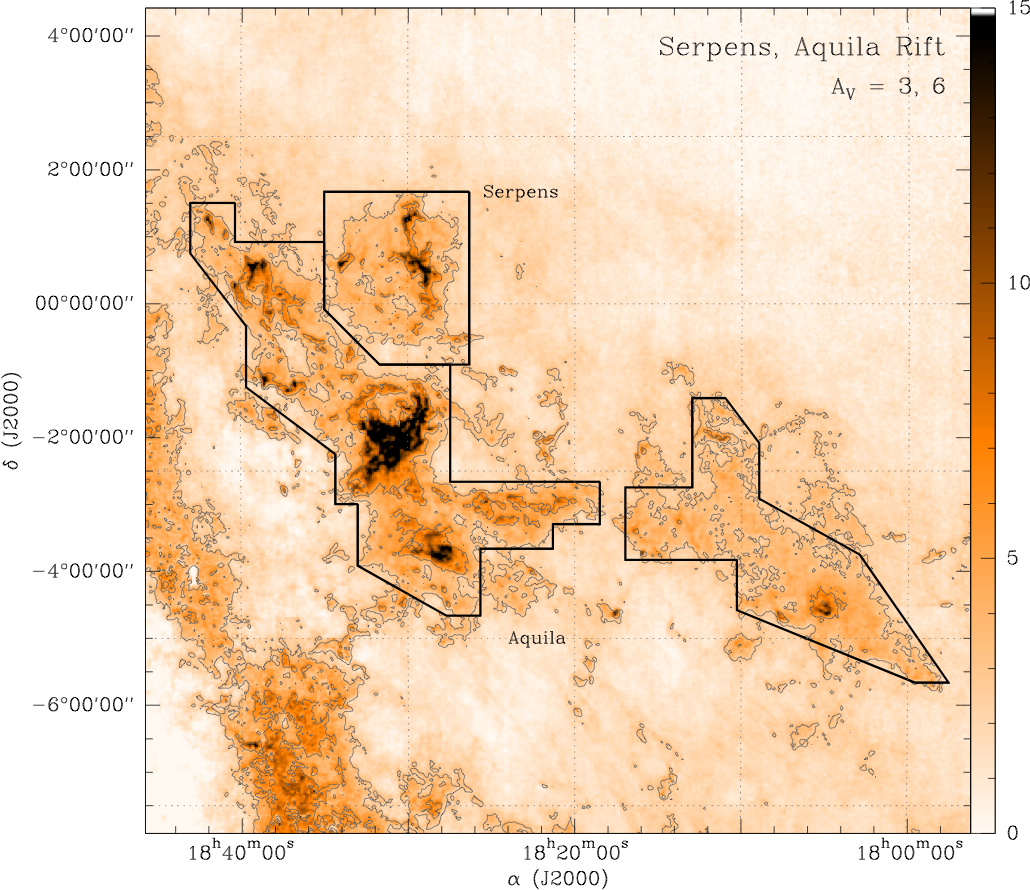
\includegraphics[width=0.6\linewidth]{gb_serpens.jpg}}
\hfill
\caption{Туманность в созвездии Змея, изображение от космического телескопа Гершель (Hershel)}
\label{fig:area}
\end{figure}


Расстояние до туманности оценивается по-разному. Та её часть, которая относится к созвездию Орёл, расположена на расстоянии 225$\pm$55 парсек от Земли. Область, относящаяся к Змее, несколько дальше. Согласно измерениям параллакса, проведённым на радиоинтерферометре VLBA, она находится на расстоянии 415$\pm$25 парсек[ссылка та же].

Несмотря на то, что исследуемая область известна наличием звездообразования, ни одна звезда в ней не идентифицирована как относящаяся к типу Т Тельца. Это связано с расположением туманности близко к галактической плоскости и недостатком наблюдений в нужных спектральных диапазонах.

Мы рассматривали область неба, для которой прямое восхождение лежит в интервале от 17.96 до 18.72, а наклонение от -5 до 5.5. Вторая часть туманности не рассматривалась из-за отсутствия необходимых наблюдений.

\section{Метод поиска}

По фотометриям galex, цветовым диаграммам + отсев по собственным движениям, эффективным температурам и simbad.

\section{Актуальность}

О космическом телескопе Спектр-УФ. Неисследованная область

\chapter{T Tauri}
\input{T Tauri}




\addcontentsline{toc}{chapter}{\bibname}

\bibliography{bibliography}     %% имя библиографической базы (bib-файла) 

\end{document}